%!TEX encoding = IsoLatin
%!TEX main = ../../main.tex

The idea of a Self-Sovereign-Identity as a Service is to support a constrained device to create and manage its self-sovereign-identity. Since IoT devices cannot run natively the complete SSI stack there is a need to design and develop an edge device capable of providing such an identity to constraint devices as a service.  Such a solution has the advantage of increasing the number of devices that can interact in such a secure digital ecosystem.

\section{Use case analysis}
The first step is to analyse and identify critical cryptographic operations involved in self-sovereign-identity management. The examples in figures \ref{usecase-did}, \ref{usecase-issuer} and \ref{usecase-verifier} illustrate in a high-level way how to create and use verifiable credentials. 
\begin{figure}[!h]
    \centering
    \includesvg[inkscapelatex=false, scale=0.80]{./chapters/images/use-case-did_creation.svg}
    \caption{Creation of a DID}
    \label{usecase-did}
\end{figure}

\subsection{Creation of a DID}
Independently from the chosen registry, when a holder creates a DID, he uniquely binds cryptographic proofs with the DID identifier. In this process, the holder typically needs to generate public-private key pairs and then insert them in the DID document. The order of operations can be seen in figure \ref{usecase-did}. 
\subsection{Verifiable Credential Issuance}
\begin{figure}[!h]
    \centering
    \includesvg[inkscapelatex=false, scale=0.80]{./chapters/images/use-case-credential_creation.svg}
    \caption{Issuance - verifiable credential creation}
    \label{usecase-issuer}
\end{figure}
Next, a holder can get a verifiable credential from an issuer, that will verify the identity in some way, for example by examining some provided documentation. If the requirements are satisfied, the issuer will generate a verifiable credential by linking her identity information to DID. The holder receiving the verifiable credential will verify its validity and save it in his personal credential repository. All of this is shown in figure \ref{usecase-issuer}. 
\subsection{Verifiable Credential Verification}
\begin{figure}[!h]
    \centering
    \includesvg[inkscapelatex=false, scale=0.80]{./chapters/images/use-case-credential_usage.svg}
    \caption{Verification - verifiable credential usage}
    \label{usecase-verifier}
\end{figure}

Moreover, as can be seen in figure \ref{usecase-verifier}, once a holder has a DID and a verifiable credential, he can use them to access a service to a verifier. The holder will use the DID to prove to the requesting party that it is the controller of that DID through some sort of challenge-response. Then, the holder will create a verifiable presentation starting from one or more verifiable credentials. If possible, it is recommended to use selective disclosure, i.e. presenting proofs of claims without revealing the entire verifiable credential, to reduce correlation. Once created the verifiable presentation the holder can send it to the verifier and he will check its validity and authorize the holder if everything is fine.  
\section{Performance analysis}
After analysing the different use cases, as highlighted in figures \ref{usecase-did}, \ref{usecase-issuer} and \ref{usecase-verifier}, the cryptographic operations that could be  critical for a constrained device are:
\begin{itemize}
    \item keys generation
    \item signature generation and verification
    \item proof generation and verification
\end{itemize}

To understand how much critical these operations are on a constrained device it is necessary to analyse the differences between a non-constrained one by getting their execution times and comparing the result. 
STM32L4+ Discovery kit IoT node\cite{stm32-board-product} has been used as a constrained device equipped with the \texttt{STM32L4S5 MCU @ 120 MHz}, 2 Mbytes of flash memory and 640 Kbytes of SRAM. While, as a non-constrained device, which has also been called \textit{edge device}, has been used a server with an \texttt{Intel Xeon Silver 4110 CPU @ 2.10GHz}. 

\begin{figure}[h!]
    \centering
    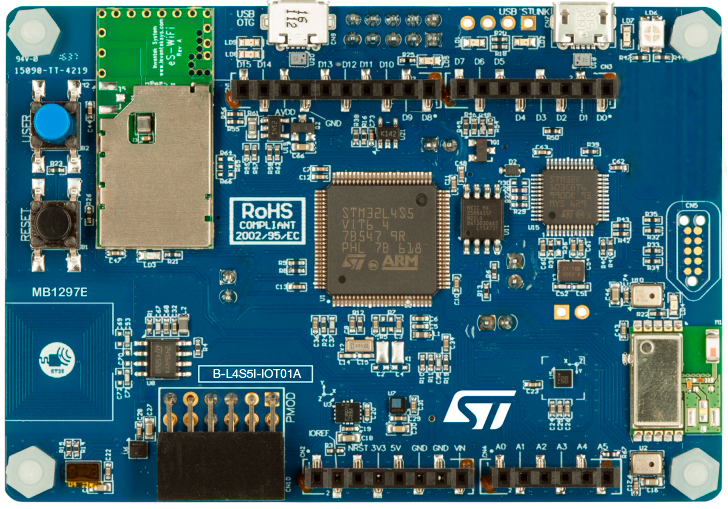
\includegraphics[scale=0.30]{./chapters/images/STM32L4+ Discovery kit IoT node.jpeg}
    \caption{STM32L4+ Discovery kit IoT node\cite{stm32-board-product}.}
    \label{stm-board}
\end{figure}

\textit{Mbed TLS} has been used as a library that implements the operation for key generation and signature (generation and verification). Mbed TLS is a C library that implements cryptographic primitives, it supports RSA, ECDSA, and other algorithms such as Ed25519. It has a small code footprint which makes it reasonable to use for embedded systems \cite{mbed-tls}. To test if a constrained device could be capable to implement and use some \textit{zero-knowledge proof} mechanisms, it has been decided to use a library which implements the BBS\texttt{+} signature scheme \cite{bbsplus}. BBS\texttt{+} signatures can be used to generate signature proofs of knowledge and selective disclosure zero-knowledge proofs \cite{bbs-rust} and they are implemented on top of BLS12-381 elliptic curve \cite{bls-curve}, which is a curve not supported in Mbed TLS. Since available BBS\texttt{+} libraries are also not supported for STM32L4, it has been decided to take execution times only on the edge device. Then execution times between the ECDSA signature scheme and BBS\texttt{+} signature scheme are comparable since they are been taken on the same architecture and they are both elliptic curve signature schemes.

\section{Results}
It is evident from the table \ref{time-table1} that RSA is usable on constrained devices in real-life applications only if the key generation is precomputed, otherwise is unusable. On the constrained device, RSA signing and verification are faster than ECDSA, but ECDSA provides the same level of security as RSA but it does so while using much shorter key lengths. In applications where it could be useful to generate a keypair on the fly, ECDSA is a must. On the edge device, the ECDSA signing operation is faster than RSA, while the RSA verification process is faster than ECDSA.  It can also be noted that the time difference between the constrained device and the edge device is huge, probably due to the frequency of operation of the MCU and the CPU.

\begin{table}[!h]
    \centering
    \begin{tabular}{| l || r | r | r |}
        \hline      
        \textbf{Operation} & \textbf{constrained device}$^\star$ & \textbf{edge device}$^\star$ \\ [0.5ex] 
        \hline \hline 
        EC-p256-keygen                  & 318 ms  & 0.5 ms \\
        \hline
        ECDSA-p256-SHA256-sign          & 1\,503 ms & 0.6 ms \\
        \hline
        ECDSA-p256-SHA256-ver           & 6\,031 ms & 2.0 ms \\
        \hline \hline
        RSA2048-keygen                  & 622\,749 ms  & 186  ms \\
        \hline
        RSA2048-SHA256-sign          & 1\,305 ms & 3.60 ms \\
        \hline
        RSA2048-SHA256-ver           & 331 ms & 0.07  ms \\
        \hline
    \end{tabular}\\
    \footnotesize $^\star$mbedTLS library
    \caption{Execution time comparison between constrained and non-constrained devices}
    \label{time-table1}
\end{table}

Furthermore, in table \ref{time-table2} ECDSA signatures and BBS\texttt{+} signatures are compared on the same CPU architecture. The obtained results are that BBS\texttt{+} signature scheme is much slower than the ECDSA one, even if they are both elliptic curve based. The order of magnitude of the percentage increase is 3, which is a significant difference. 
   
\begin{table}[!h]
    \centering
    \begin{tabular}{| l || r | r | r|}
        \hline 
        \textbf{Operation} & \textbf{ECDSA}$^\star$ & \textbf{BBS\texttt{+}}$^\star$$^\dagger$ & \textbf{\% increase} \\ [0.5ex] 
        \hline  \hline 
        keygen   & 0.2   ms      & 39 ms   &\texttt{+}7\,800\\
        \hline
        sign     & 0.6   ms      & 27  ms   &\texttt{+}4\,500\\
        \hline
        verify   & 2.0  ms         & 166 ms   &\texttt{+}8\,300\\
        \hline
    \end{tabular}
    \\
    \footnotesize $^\star$Xeon 2.10GHz \enspace\enspace $^\dagger$Rust bbs library
    \caption{Execution time comparison between ECDSA and BBS\texttt{+}}
    \label{time-table2}
\end{table}

\section{Design and implementation choices}
The obtained results suggest that a constrained device cannot use the BBS\texttt{+} signature scheme in real-world applications, since it can be supposed that execution times will be considerably high. In the Self-sovereign Identity as a Service (SSIaaS) paradigm, a new role is defined, called edge. The edge device interacts with a constrained IoT object and provides functionalities to create and support it in identity management, this can be seen in figure \ref{poc-design}. The identified and exposed operations by the edge device are:
\begin{itemize}
    \item key pairs generation
    \item storage of a verifiable credential
    \item generation of a verifiable presentation
\end{itemize}

\subsection{Self-Sovereign-Identity as a Service Ecosystem}

\begin{figure}[!h]
    \centering
    \includesvg[inkscapelatex=false, scale=1]{./chapters/images/poc.svg}
    \caption{Basic components of Self-Sovereign-Identity as a Service}
    \label{poc-design}
\end{figure}

From now on, the focus is on the interaction between the edge device and the IoT-constrained node. The IoT device can request the edge node to generate key pairs that could later use to generate a verifiable presentation. The IoT device can store on the edge node a verifiable credential got from an issuer. If the IoT device what to interact with a verifier, it has to provide a verifiable presentation, which is generated by the edge device starting from the verifiable credential and signing the vc with a keypair previously generated for that specific IoT client. 
Since these are security-critical operations because they handle the identity of the IoT node, it needs the guarantee that the data shared with the edge device and the executed code are protected with respect to confidentiality and integrity. Hence, a TEE has been implemented using the keystone framework.  Figures \ref{manufacturer-provisioning} and \ref{poc-architecture} show the architecture and the preliminary interactions between the IoT device and the edge device before the constrained device can ask for services. Figures \ref{poc-gen-keys}, \ref{poc-store-vc} and \ref{poc-get-vp} show in a top-level way how the operations have been implemented. 

\subsection{IoT Device Provisioning}

The first step before deploying an IoT device in the network is its provisioning. Provisioning means configuring the IoT device to be ready when joining the network to communicate with and be authenticable by the edge device. In the implemented solution, a trustworthy system administrator provisions the client, i.e., the constrained device, with: 
\begin{itemize}
    \item a key pair (client secret and public keys) used to authenticate itself to the server, i.e., the edge device
    \item expected security monitor and enclave hashes to verify that the edge device is running the expected application in the enclave 
    \item the device public key of the edge device to verify that is running on trusted hardware
\end{itemize} 

\begin{figure}[!h]
    \centering
    \includesvg[inkscapelatex=false, scale=0.7]{./chapters/images/manufacturer.svg}
    \caption{Manufacturer provisions device with expected hashes, keys and signature of the public key}
    \label{manufacturer-provisioning}
\end{figure}

Then, the system administrator signs the public key of the IoT client and saves the signature. The signature is verifiable with the public key of the system administrator. It proves (trust assumptions) that the device with access to the client's secret belongs to a recognised IoT network group. This client authentication method was chosen because the edge device only needs to retain the system administrator's public key in memory, rather than keeping track of all the clients' public keys in a database to determine whether a client is authorized to access services.

\subsection{Attestation Report and Session Context}
With the use of ed25519 signatures on hashes of the security monitor and enclave content, Keystone supports a basic attestation mechanism, as introduced in section \ref{keystone-components}. Once an enclave has started the execution, it requests the SM to generate a signed enclave report and a signed SM report. The SM Report enclose a hash of the security monitor and the attestation public key, all signed by the device root key. The enclave report consists of a hash of the enclave at initialization and a data block from the enclave of up to 1Kbytes, 
all signed by the attestation public key. A verifier, in this case, the IoT device when provided with the device public key, expected SM hash, and expected enclave hash will verify the signatures of these reports. An example of an attestation report is shown in listing \ref{attestation-report}. \\

\begin{lstlisting}[caption={Example of a attestation report  generated by the enclave},captionpos=b,style=json, label={attestation-report},frame=single]
{
    "enclaveApplication": {
        "hash": "11ff35526c90c469ca6878dc22494703c554db654...",
        "enclaveData": "b07dfd3047fb5213b8af9b76594a06891...",
        "signature": "58ca380c6b4476ed7b27143d92dec14fff2858ffef8ed6ef4..."
    },
    "securityMonitor": {
        "hash": "e51749130b6036fe85b27409a4ea3e1c078fe4dcb76...",
        "publicKey": "cd98f4a28a8523ba8ecd31175aa0e2330b2f46e70...",
        "signature": "e738f4e708f73ffa4a0d3dc2199c9e0ac119bf14b32da33a..."
    },
    "devicePublicKey": "0faad4ff01178583baa588966f7c1ff32564dd17d..."
}
\end{lstlisting}

When designing the demo, the session context has been introduced to authenticate the client on the server side. The session context includes two sections: the stub certificate and the homonym session context. The first one contains the client's public key and the signature of the client's public key, made at the provisioning phase by the system administrator and verifiable with the public root key. The enclosed session context contains a data block, all signed by the client public key. A verifier, in this case, the edge node when provided with the root public key of the system administrator will verify the signatures of this structure. An example of a session context is shown in listing \ref{session-context}. \\

\begin{lstlisting}[caption={Example of a session context generated by the client},captionpos=b,style=json, label={session-context},frame=single]
{
    "sessionContext": {
        "data": "3a2992fe52a2082b26f8009117be53decff68...",
        "dataSignature": "02b0b554aecd929419a6c525ebfde..."
    },
    "stubCertificate": {
        "clientPublicKey": "e95f84f09574d8fe73c0e692905c6c8d...",
        "rootSignature": "a8b20a77877b79ca0d699091f8b303463b..."
    }
}
\end{lstlisting}

In the demo implementation, the data part of the session context and the attestation report are both used for the Diffie-Hellman key exchange protocol so that the two parties can securely compute a shared key for creating a secure encrypted channel. 

\subsection{Demo Architecture}
In the following description, the implemented architecture has been simplified for development reasons. This demo demonstrates how a remote (constrained) device can request computation to be performed on an untrusted server using an enclave. (The demo uses test keys, it is not safe and should not be used in production). The demo architecture consists of:
\begin{itemize}
    \item a server enclave application and an untrusted host application hosted on a RISC-V processor
    \item an IoT client provisioned by the system administrator  
\end{itemize} 

The demo enclave application has essential enclave capabilities (attestation report generation, data sealing, etc.), uses \texttt{libsodium} for establishing a secure channel and exposes three SSI-related services. The untrusted enclave host serves a few functions: starting the enclave, proxying network packets from and to the client and storing sealed data. The remote client establishes a connection with the untrusted host, verifies the enclave report, transmits the session context, and creates a secure channel before being able to communicate with the host to request offloaded computations. 

\begin{figure}[!h]
    \centering
    \includesvg[inkscapelatex=false, scale=0.7]{./chapters/images/Demo architecture3.svg}
    \caption{Demo architecture}
    \label{poc-architecture}
\end{figure}

\subsubsection{Running the demo}

At the start, the client will connect to the enclave and perform the remote attestation. Expected hashes in the attestation report will be used by the trusted client to verify that the enclave is created with the right application and initialized by the known version of the security monitor. If the attestation is successful, the client can send its attestation, also called session context. The server will check the signature validity provided by the client, verifying it with the public key of the system administrator (\texttt{root\_pk}). On the contrary, if the edge device attestation report is invalid, the client will close the connection. (For instance, you could pass a flag when launching the client to ignore the attestation report of the server for testing purposes or during development when changing the enclave application).
Upon exchanging the session context and the attestation report, they establish a secure channel and the enclave-host waits for messages.

\subsection{Offloaded Operations}
Once the edge node and the constrained devices have established a secure channel to communicate, the enclave waits for the client to request service. Once a message is received, the enclave authenticates and decrypts the message. If successful, it processes the message and passes the request to a specific \textit{ocall}, i.e, \texttt{ocall\_wait\_for\_request(...)}, which dispatches the requests proxied by the untrusted host coming from the client. By checking the request type, the enclave understands what service the client has requested. After processing the request, the enclave returns the result through the secure channel.

\subsubsection{Setup phase}
Using Keystone SDK, generated sealing key size will be 128 bytes. In the demo implementation, the sealing key is used as a seed for generating an ed25519 key pair. The sealed data are signed with the ed25519 key pair. Whereas, the key used for encryption consists of the first \texttt{crypto\_aead\_chacha20poly1305\_KEYBYTES} bytes, i.e. 32 bytes. of the sealing key. As is visible in the listing \ref{setup-seal-material}, \textit{libsodioum} \cite{libsodium} is used for generating these keys, which is a cryptographic library written in C. \\

\begin{lstlisting}[caption={Setup of the encryption key and ed25519 keypair},captionpos=b,label={setup-seal-material},language=C,frame=single]
// here sealing_key is used as a seed to gen sign keys
crypto_sign_seed_keypair(enclave_signing_pk, enclave_signing_sk,
                            sealing_material.key);

// sealing key here is used for the data encryption usage
memcpy(enc_key, sealing_material.key, crypto_aead_chacha20poly1305_KEYBYTES); 
\end{lstlisting}

\begin{figure}[!h]
    \centering
    \includesvg[inkscapelatex=false, scale=0.7]{./chapters/images/poc-keys.svg}
    \caption{Key pairs generation operation (pseudo-code)}
    \label{poc-gen-keys}
\end{figure}

\subsubsection{Generate public keys}
Consider the service of key pairs generation. The client sends this request along with the key type and a secret. The server process the incoming request. It generates the sealing key, using as an identifier in the key derivation function the client's public key and the secret sent by the client. Then, it generates two key pairs of the type that the client indicates in the request. (For demo purposes only \texttt{EdDSA} can be generated, in future \texttt{BBS+} signature scheme will be implemented). 
Next, it encrypts the generated key pair with the obtained sealing key and signs the obtained ciphertext with an enclave signing key. Next, the enclave application calls \texttt{ocall\_save\_sealed\_data(...)}, which is the edge wrapper function to the system-call \texttt{ocall(OCALL\_SAVE\_SEALED\_DATA, buffer, len, 0, 0)}. This call exports the buffer, containing the ciphertext and the signature of the generated key pairs, from the enclave to be stored in the untrusted non-volatile memory by the host process. The file name is composed of the public key of the client and the type of data saved, in this case, keys, so, for example, the file name will be \texttt{<client\_pub\_key>\_keys}. The host saves the data obtained from the enclave and returns the control. 
Finally, the enclave sends back to the client the response, which will contain only the public part of the generated keys. 

\subsubsection{Store verifiable credential}
Consider the service of storing a verifiable credential. The client sends this request along with the verifiable credential and a secret. The server process the incoming request. It generates the sealing key, using as an identifier in the key derivation function the client's public key and the secret sent by the client. (The sealing key will be equal for the same client). Then, it encrypts the received verifiable credential with the obtained sealing key and signs the obtained ciphertext with an enclave signing key. Next, the enclave application calls \texttt{ocall\_save\_sealed\_data(...)}, which is the edge wrapper function to the system-call \texttt{ocall(OCALL\_SAVE\_SEALED\_DATA, buffer, len, 0, 0)}. This call exports the buffer, containing the ciphertext and the signature of the verifiable credential, from the enclave to be stored in the untrusted non-volatile memory by the host process. The file name is composed of the public key of the client and the type of data saved, in this case, a verifiable credential, so, for example, the file name will be \texttt{<client\_pub\_key>\_vc}. The host saves the data obtained from the enclave and returns the control. 
Finally, the enclave sends back to the client the response, which will contain in this case only a \texttt{SUCCESS} flag. \\

\begin{figure}[!h]
    \centering
    \includesvg[inkscapelatex=false, scale=0.7]{./chapters/images/poc-vc.svg}
    \caption{Storage of a verifiable credential operation (pseudo-code)}
    \label{poc-store-vc}
\end{figure}
\subsubsection{Get verifiable presentation}
Consider the service of generating a verifiable credential. The client sends this request along with a nonce and a secret. The server process the incoming request. It generates the sealing key, using as an identifier in the key derivation function the client's public key and the secret sent by the client. (The sealing key will be equal for the same client). Then, the enclave application calls \texttt{ocall\_retrieve\_sealed\_data(...)}, which is the edge wrapper function to the system-call \texttt{ocall( OCALL\_RETRIEVE\_SEALED\_DATA, buffer, len, msg, sizeof( struct edge\_data ))}. This call exports the buffer, containing the file name to be retrieved, and the host once read the correct file copies it into the shared memory region, sets the \textit{edge\_call} return status to SUCCESS and returns control to the enclave. The host saves the data obtained from the enclave and returns the control. The runtime copies the file from the shared region into return buffers and then resumes the enclave ocall wrapper code.
The function will be executed for retrieving from the untrusted non-volatile memory the verifiable credential (the file name will be \texttt{<client\_pub\_key>\_vc}) and for retrieving the previously generated keys (the file name will be \texttt{<client\_pub\_key>\_keys}).
The enclave will check the validity of signatures and decrypt the sealed data.  
Finally, the enclave using the retrieved keys signs the verifiable credential with the nonce received from the client and sends back the response, which will contain a freshly generated verifiable presentation. \\

\begin{figure}[!h]
    \centering
    \includesvg[inkscapelatex=false, scale=0.7]{./chapters/images/poc-vp.svg}
    \caption{Generation of a verifiable presentation operation (pseudo-code)}
    \label{poc-get-vp}
\end{figure}

